% Copyright (C) 2010, 2013  Martin Lambers <marlam@marlam.de>
%

\documentclass[a4paper,11pt]{article}
\usepackage[english]{babel}
\usepackage{mathptmx}
\usepackage{graphicx}
\usepackage[utf8]{inputenc}
\usepackage[T1]{fontenc}
\usepackage{hyperref}

\hypersetup{
    pdftitle={The Generic Tagged Array File Format},
    pdfsubject={Specification},
    pdfauthor={Martin Lambers},
    pdfborder={0 0 0}
}

\pagestyle{empty}

\newcommand{\code}[1]{\texttt{#1}}

\begin{document}

\title{The Generic Tagged Array File Format}
%\author{Martin Lambers}
\author{~}
%\date{}%
\date{~}
\maketitle

\noindent
{\scriptsize
Copyright (C) 2010, 2013 Martin Lambers\\~\\
Permission is granted to copy, distribute and/or modify this document
under the terms of the GNU Free Documentation License, Version 1.2 or
any later version published by the Free Software Foundation; with no
Invariant Sections, no Front-Cover Texts, and no Back-Cover Texts.
%A copy of the license is included in the section entitled ``GNU Free
%Documentation License''.
}


\phantomsection 
\addcontentsline{toc}{section}{Changes}
\section*{Changes}

\begin{itemize}
\item \textbf{2013-02-06} Fixed typos.
\item \textbf{2010-08-17} Remove the meaning of the second lowest bit in the
flag byte of the header. The same information can be extracted from the sixth
header byte instead. This allows to simplify the libgta API. Compatibility with
older libgta versions is retained.
\item \textbf{2010-06-06} Various extensions, cleanups, clarifications.
The list of reserved tags was moved to an external file because it may change
while the file format itself remains unchanged.
\item \textbf{2010-04-16} Initial version.
\end{itemize}


\phantomsection 
\addcontentsline{toc}{section}{Introduction}
\section*{Introduction}

This document specifies version 1 of the Generic Tagged Array (GTA) file format.
This file format has the following features:
\begin{itemize}
\item GTA files can store any kind of data in multidimensional arrays
\item GTA files can use simple tags to describe the data
\item GTA files are streamable, which allows direct reading from and
	writing to pipes, network sockets, or other non-seekable media
\item GTA files can optionally use ZLIB, BZIP2, or XZ compression,
	allowing a tradeoff between compression/decompression speed and
	compression ratio
\item Uncompressed GTA files allow easy out-of-core data access
\end{itemize}


\section{Definitions}

\subsection{Arrays}

An array has zero or more \emph{dimensions}, and a size of at least one in each
dimension. These dimension sizes determine the number of array elements.
An array element consists of zero or more \emph{components}.
Each component has a \emph{type}. The types are defined in table~\ref{tab:types}.
The special type \code{GTA\_BLOB} allows the user to define custom types
of arbitrary length.

\begin{table}
\begin{tabular}{l|r|r|p{.55\textwidth}}
Type & No. & Bytes & Description\\\hline
\code{GTA\_INT8}      &  1 & 1		& C99 \code{int8\_t}		\\
\code{GTA\_UINT8}     &  2 & 1 		& C99 \code{uint8\_t}		\\
\code{GTA\_INT16}     &  3 & 2 		& C99 \code{int16\_t}		\\
\code{GTA\_UINT16}    &  4 & 2 		& C99 \code{uint16\_t} 	\\
\code{GTA\_INT32}     &  5 & 4 		& C99 \code{int32\_t}		\\
\code{GTA\_UINT32}    &  6 & 4 		& C99 \code{uint32\_t}		\\
\code{GTA\_INT64}     &  7 & 8 		& C99 \code{int64\_t} 		\\
\code{GTA\_UINT64}    &  8 & 8 		& C99 \code{uint64\_t}		\\
\code{GTA\_INT128}    &  9 & 16		& C99 \code{int128\_t} (unavailable on many platforms)		\\
\code{GTA\_UINT128}   & 10 & 16		& C99 \code{uint128\_t} (unavailable on many platforms)		\\
\code{GTA\_FLOAT32}   & 11 & 4 		& IEEE 754 single precision floating point (on many platforms: \code{float}) \\
\code{GTA\_FLOAT64}   & 12 & 8 		& IEEE 754 double precision floating point (on many platforms: \code{double}) \\
\code{GTA\_FLOAT128}  & 13 & 16		& IEEE 754 quadrupel precision floating point (unavailable on many platforms, even if \code{long double} exists) \\
\code{GTA\_CFLOAT32}  & 14 & 8		& complex (re,im) based on \code{GTA\_FLOAT32} \\
\code{GTA\_CFLOAT64}  & 15 & 16		& complex (re,im) based on \code{GTA\_FLOAT64} \\
\code{GTA\_CFLOAT128} & 16 & 32		& complex (re,im) based on \code{GTA\_FLOAT128} \\
\code{GTA\_BLOB}      &  0 & ---    	& Data blob; must be endianness-independent; user must specify the size \\
\end{tabular}
\caption{GTA data types. All integer types use the common two-complement
representation. All floating point types conform to IEEE 754. A corresponding
C99 type might not exist on all platforms.}
\label{tab:types}
\end{table}

For example, an image with $640\times 480$ pixels in the common RGB format
would have two dimensions, the first with size 640, the second with size 480.
Each array element would consist of three components, all of type
\code{GTA\_UINT8}.


\subsection{Tags}
\label{sec:tags}

A \emph{tag} consists of a tag name and a tag value.

A tag name is a non-empty, zero-terminated, \mbox{UTF-8} encoded string that does not
contain control characters (characters with a code less than 32 or equal to 127)
and does not contain the character \code{=}.

A tag value is a zero-terminated, \mbox{UTF-8} encoded string that does not contain
control characters (characters with a code less than 32 or equal to 127). It can
be empty, and it can contain the character \code{=}.

Leading or trailing white space is not ignored; it is part of the name or
value string.

A \emph{tag list} consists of zero or more tags.

An array has multiple tag lists:
\begin{itemize}
\item One global tag list, containing tags that are relevant to the array as a
whole.
\item A dimension tag list for each dimension, containing tags that are
relevant to this particular dimension.
\item A component tag list for each element component, containing tags that
are relevant to this particular component.
\end{itemize}

An array does not need to have any tags in its tag lists. If it does have
tags, these are subject to certain rules, see the external documentation about
reserved tags.

For example, an image might have a global tag list containing the tag\linebreak
\code{DATE=Fri,~~4~Dec~2009 22:29:43 +0100 (CET)}, 
a tag list for the first dimension containing the tag \code{INTERPRETATION=X},
a tag list for the second dimensions containing the tag
\code{INTERPRETATION=Y}, and three component tag lists, containing the tags
\code{INTERPRETATION=SRGB/RED}, \code{INTERPRETATION=SRGB/GREEN},\linebreak
\code{INTERPRETATION=SRGB/BLUE} respectively.


\subsection{Chunks}

A \emph{chunk} stores a number of chunk data bytes, either compressed or uncompressed.
It begins with a chunk header, defined as follows:
\begin{itemize}
\item The first 8 bytes of the chunk header contain a value of type \code{GTA\_UINT64},
subject to the endianness type of the file (see next section for details).
This value is the number of bytes of the chunk data (excluding the
header). Currently, it is limited to $2^{24}$, so that a chunk cannot store more
than 16 MiB.
\item Only if the previous value is not zero, the next byte of the chunk
contains a value of type \code{GTA\_UINT8}.  This value specifies the
compression method of the chunk, as defined in Tab.~\ref{tab:compression}.
\item Only if the compression method is not \code{GTA\_NONE}, the next 8 bytes
contain a value of type \code{GTA\_UINT64}, subject to the endianness type of
the file. This value is the number of bytes that the compressed chunk data
uses. It is guaranteed to be less than or equal to the number of bytes of the
chunk data. If a compression method would produce compressed chunk data that
is larger than the uncompressed chunk data, the chunk is simply not compressed
but stored uncompressed (with the compression method \code{GTA\_NONE}).
\end{itemize}

\begin{table}
\begin{tabular}{l|l|l}
Compression method & Number & Description\\\hline
\code{GTA\_NONE}  & 0 & No compression \\
\code{GTA\_ZLIB}  & 1 & ZLIB compression with default level (fast,\\
                  &   & moderate compression ratio) \\
\code{GTA\_ZLIB1} & 4 & ZLIB compression with level 1\\
\code{GTA\_ZLIB2} & 5 & ZLIB compression with level 2\\
\code{GTA\_ZLIB3} & 6 & ZLIB compression with level 3\\
\code{GTA\_ZLIB4} & 7 & ZLIB compression with level 4\\
\code{GTA\_ZLIB5} & 8 & ZLIB compression with level 5\\
\code{GTA\_ZLIB6} & 9 & ZLIB compression with level 6\\
\code{GTA\_ZLIB7} & 10& ZLIB compression with level 7\\
\code{GTA\_ZLIB8} & 11& ZLIB compression with level 8\\
\code{GTA\_ZLIB9} & 12& ZLIB compression with level 9\\
\code{GTA\_BZIP2} & 2 & BZIP2 compression (moderate speed,\\
                  &   & good compression ratio) \\
\code{GTA\_XZ}    & 3 & XZ compression (low compression speed,\\
                  &   & moderate decompression speed,\\
		  &   & good or very good compression rates) \\
\end{tabular}
\caption{GTA compression methods.}
\label{tab:compression}
\end{table}

After the chunk header (8, 9, or 17 bytes, depending on the chunk data size
and compression method), the chunk data follows, either uncompressed, using
the number of bytes given in the first header value, or compressed, using
the number of bytes given in the third header value.

A \emph{chunk list} is a list of one or more chunks. A chunk with the chunk
data size zero marks the last chunk in a chunk list.


\section{File Format}

A GTA consists of the GTA header and the GTA data. The GTA header stores
information about the file format, the list of dimensions, the list of element
components, and all tag lists. See Sec.~\ref{sec:gta-header}.
The GTA data is stored immediately after the header. See Sec.~\ref{sec:gta-data}.


\subsection{GTA Header}
\label{sec:gta-header}

Each GTA starts with a header. The first six bytes of the header identify the
GTA version and properties. See Fig.~\ref{fig:gta-header}.

\begin{figure}
\begin{center}
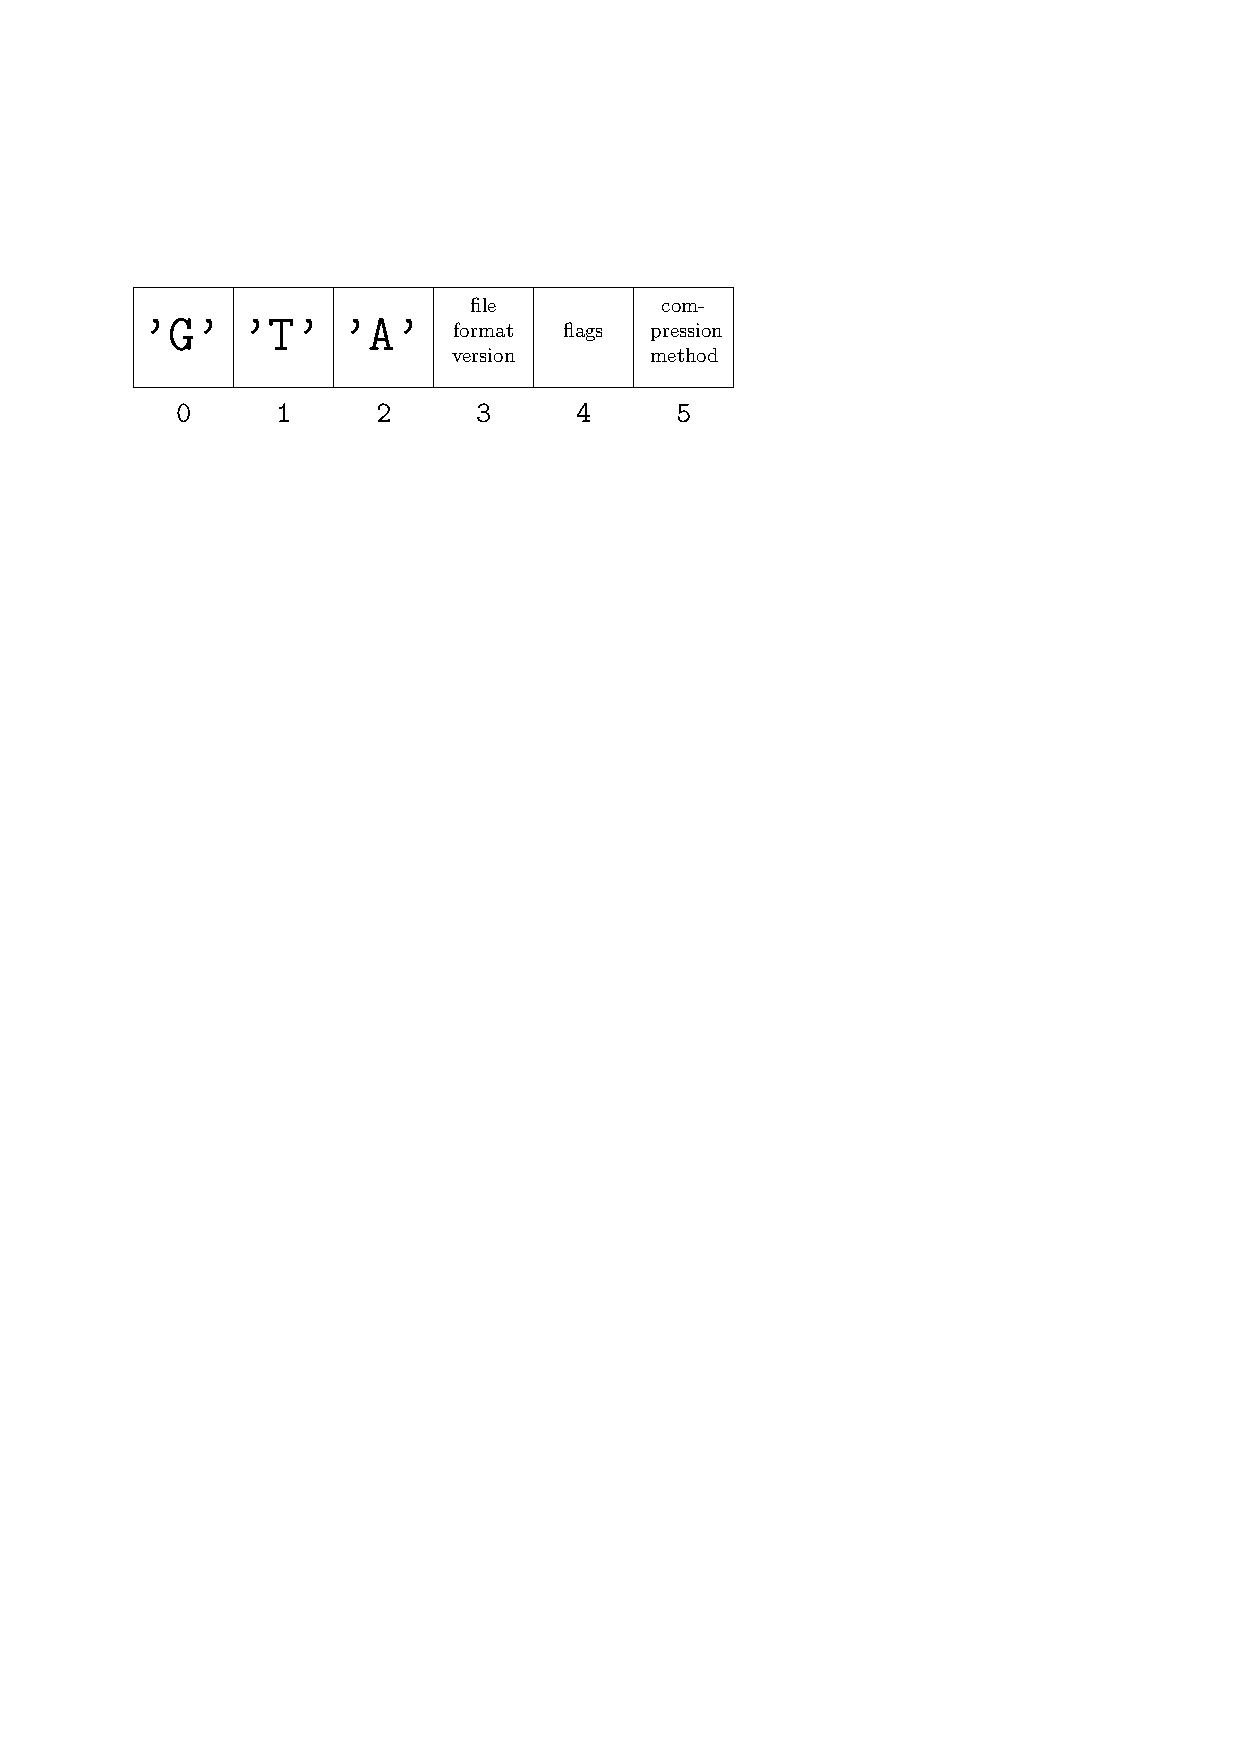
\includegraphics[width=\textwidth]{gta-header.pdf}
\end{center}
\caption{The first six bytes of a GTA header.}
\label{fig:gta-header}
\end{figure}

The first three bytes of a GTA header are of type \code{GTA\_UINT8} and contain
the \mbox{UTF-8} codes of the characters \code{G}, \code{T}, and \code{A}.

The fourth byte is of type \code{GTA\_UINT8} and contains the GTA file format
version number. Currently, this value must always be 1.

The fifth byte is of type \code{GTA\_UINT8}, and each bit represents a flag that
can be set (1) or unset (0).

The lowest bit flag determines if multibyte values in the file are in big endian
(1) or little endian (0) byte ordering. This flag applies to all values in the
header and in the data. (The array element component type \code{GTA\_BLOB} is special:
it must be independent of byte ordering, so that it is valid regardless of this
flag.)

The second lowest bit used to have a meaning in previous versions of this
specification. For compatibility reasons, this flag must be ignored when
reading a GTA. When writing a GTA, it must be unset (0) if the value
\code{GTA\_NONE} is stored in the sixth header byte (described below), and it
must be set (1) otherwise.

All six remaining bit flags are reserved and must currently always be unset (0).

The sixth byte in the header is of type \code{GTA\_UINT8} and contains a
recommendation for the compression type of the GTA, which must be one of the
values defined in Tab.~\ref{tab:compression}.

If this value if \code{GTA\_NONE}, then the GTA data must not be stored in
chunks. If this value is not \code{GTA\_NONE}, then the GTA data must be stored
in chunks.

This value sets the recommended compression method for all following chunks
in the GTA (header or data), but note that each chunk uses its own compression
method which may differ from this recommendation.

At byte 7 of the header, a chunk list starts. This chunk list contains the
information described in the next paragraphs.

The first information in the chunk list is the list of element components. It
consists of zero or more component definitions. A component definition starts
with one byte of type \code{GTA\_UINT8} that contains one of the values
defined in Tab.~\ref{tab:types}. If the type is \code{GTA\_BLOB}, then the
component definition contains additional 8 bytes of type \code{GTA\_UINT64}
(subject to the endianness type of the GTA). This additional value stores the
size in bytes of the component. A component definition that contains the
special value 255 in its type field signals the end of the component list.

After the list of element components, the list of dimensions is stored.  This
list consists of zero or more dimension definitions. A dimension definition
consists of 8 bytes of type \code{GTA\_UINT64} (subject to the endianness type
of the GTA). This value stores the size of the dimension, and must be greater
than zero. A dimension definition that stores the special value 0 in its size
field signals the end of the dimension list.

After the list of dimensions, the global tag list is stored.  The global tag
list stores each tag name and its tag value as-is (\mbox{UTF-8} strings, zero
terminated). An empty name (consisting only of the value 0) signals
the end of the global tag list.

After the global tag list, the tag lists of all element components follows, and
after that the tag lists of all dimensions. These tag lists are stored in the
same manner as the global tag list.

After these tag list definitions, the GTA header chunk list ends, i.e.~a
single zero-sized chunk must signal the end of the header chunk list.

The GTA array data follows immediately after the header.


\subsection{GTA Data}
\label{sec:gta-data}

The array data itself is stored in a compact form without alignment offsets or
other fill bytes of any kind. The linear format of a multidimensional array is
the same as that of a C array when the first dimension is specified last
(row-major for two-dimensional data). The following is an example for a
three-dimensional array: \code{element\_type array[size2][size1][size0]}.

The array data is stored as-is if the compression method recommended in the
sixth byte of the header is \code{GTA\_NONE}. Otherwise, it is stored in a chunk
list.

When stored as-is, individual data elements can easily be accessed if the input
is seekable.

Immediately after the array data, another GTA may follow.



%\newpage
%\renewcommand{\large}{\small}
%\renewcommand{\Large}{\normalsize}
%\newcommand{\chapter}[3][\relax]{\section*{#3}\footnotesize}
%% This is set up to run with pdflatex.
%---------The file header---------------------------------------------
%\documentclass[a4paper,12pt]{book}
%
%\usepackage[english]{babel} %language selection
%\selectlanguage{english}
%
%\pagenumbering{arabic}
%
%\usepackage{hyperref}
%\hypersetup{colorlinks, 
%           citecolor=black,
%           filecolor=black,
%           linkcolor=black,
%           urlcolor=black,
%           bookmarksopen=true,
%           pdftex}
%
%\hfuzz = .6pt % avoid black boxes
%           
%\begin{document}
%---------------------------------------------------------------------
\chapter*{\rlap{GNU Free Documentation License}}
\phantomsection  % so hyperref creates bookmarks
\addcontentsline{toc}{chapter}{GNU Free Documentation License}
%\label{label_fdl}

 \begin{center}

       Version 1.3, 3 November 2008


 Copyright \copyright{} 2000, 2001, 2002, 2007, 2008  Free Software Foundation, Inc.
 
 \bigskip
 
     <http://fsf.org/>
  
 \bigskip
 
 Everyone is permitted to copy and distribute verbatim copies
 of this license document, but changing it is not allowed.
\end{center}


\begin{center}
{\bf\large Preamble}
\end{center}

The purpose of this License is to make a manual, textbook, or other
functional and useful document ``free'' in the sense of freedom: to
assure everyone the effective freedom to copy and redistribute it,
with or without modifying it, either commercially or noncommercially.
Secondarily, this License preserves for the author and publisher a way
to get credit for their work, while not being considered responsible
for modifications made by others.

This License is a kind of ``copyleft'', which means that derivative
works of the document must themselves be free in the same sense.  It
complements the GNU General Public License, which is a copyleft
license designed for free software.

We have designed this License in order to use it for manuals for free
software, because free software needs free documentation: a free
program should come with manuals providing the same freedoms that the
software does.  But this License is not limited to software manuals;
it can be used for any textual work, regardless of subject matter or
whether it is published as a printed book.  We recommend this License
principally for works whose purpose is instruction or reference.


\begin{center}
{\Large\bf 1. APPLICABILITY AND DEFINITIONS\par}
\phantomsection
\addcontentsline{toc}{section}{1. APPLICABILITY AND DEFINITIONS}
\end{center}

This License applies to any manual or other work, in any medium, that
contains a notice placed by the copyright holder saying it can be
distributed under the terms of this License.  Such a notice grants a
world-wide, royalty-free license, unlimited in duration, to use that
work under the conditions stated herein.  The ``\textbf{Document}'', below,
refers to any such manual or work.  Any member of the public is a
licensee, and is addressed as ``\textbf{you}''.  You accept the license if you
copy, modify or distribute the work in a way requiring permission
under copyright law.

A ``\textbf{Modified Version}'' of the Document means any work containing the
Document or a portion of it, either copied verbatim, or with
modifications and/or translated into another language.

A ``\textbf{Secondary Section}'' is a named appendix or a front-matter section of
the Document that deals exclusively with the relationship of the
publishers or authors of the Document to the Document's overall subject
(or to related matters) and contains nothing that could fall directly
within that overall subject.  (Thus, if the Document is in part a
textbook of mathematics, a Secondary Section may not explain any
mathematics.)  The relationship could be a matter of historical
connection with the subject or with related matters, or of legal,
commercial, philosophical, ethical or political position regarding
them.

The ``\textbf{Invariant Sections}'' are certain Secondary Sections whose titles
are designated, as being those of Invariant Sections, in the notice
that says that the Document is released under this License.  If a
section does not fit the above definition of Secondary then it is not
allowed to be designated as Invariant.  The Document may contain zero
Invariant Sections.  If the Document does not identify any Invariant
Sections then there are none.

The ``\textbf{Cover Texts}'' are certain short passages of text that are listed,
as Front-Cover Texts or Back-Cover Texts, in the notice that says that
the Document is released under this License.  A Front-Cover Text may
be at most 5 words, and a Back-Cover Text may be at most 25 words.

A ``\textbf{Transparent}'' copy of the Document means a machine-readable copy,
represented in a format whose specification is available to the
general public, that is suitable for revising the document
straightforwardly with generic text editors or (for images composed of
pixels) generic paint programs or (for drawings) some widely available
drawing editor, and that is suitable for input to text formatters or
for automatic translation to a variety of formats suitable for input
to text formatters.  A copy made in an otherwise Transparent file
format whose markup, or absence of markup, has been arranged to thwart
or discourage subsequent modification by readers is not Transparent.
An image format is not Transparent if used for any substantial amount
of text.  A copy that is not ``Transparent'' is called ``\textbf{Opaque}''.

Examples of suitable formats for Transparent copies include plain
ASCII without markup, Texinfo input format, LaTeX input format, SGML
or XML using a publicly available DTD, and standard-conforming simple
HTML, PostScript or PDF designed for human modification.  Examples of
transparent image formats include PNG, XCF and JPG.  Opaque formats
include proprietary formats that can be read and edited only by
proprietary word processors, SGML or XML for which the DTD and/or
processing tools are not generally available, and the
machine-generated HTML, PostScript or PDF produced by some word
processors for output purposes only.

The ``\textbf{Title Page}'' means, for a printed book, the title page itself,
plus such following pages as are needed to hold, legibly, the material
this License requires to appear in the title page.  For works in
formats which do not have any title page as such, ``Title Page'' means
the text near the most prominent appearance of the work's title,
preceding the beginning of the body of the text.

The ``\textbf{publisher}'' means any person or entity that distributes
copies of the Document to the public.

A section ``\textbf{Entitled XYZ}'' means a named subunit of the Document whose
title either is precisely XYZ or contains XYZ in parentheses following
text that translates XYZ in another language.  (Here XYZ stands for a
specific section name mentioned below, such as ``\textbf{Acknowledgements}'',
``\textbf{Dedications}'', ``\textbf{Endorsements}'', or ``\textbf{History}''.)  
To ``\textbf{Preserve the Title}''
of such a section when you modify the Document means that it remains a
section ``Entitled XYZ'' according to this definition.

The Document may include Warranty Disclaimers next to the notice which
states that this License applies to the Document.  These Warranty
Disclaimers are considered to be included by reference in this
License, but only as regards disclaiming warranties: any other
implication that these Warranty Disclaimers may have is void and has
no effect on the meaning of this License.


\begin{center}
{\Large\bf 2. VERBATIM COPYING\par}
\phantomsection
\addcontentsline{toc}{section}{2. VERBATIM COPYING}
\end{center}

You may copy and distribute the Document in any medium, either
commercially or noncommercially, provided that this License, the
copyright notices, and the license notice saying this License applies
to the Document are reproduced in all copies, and that you add no other
conditions whatsoever to those of this License.  You may not use
technical measures to obstruct or control the reading or further
copying of the copies you make or distribute.  However, you may accept
compensation in exchange for copies.  If you distribute a large enough
number of copies you must also follow the conditions in section~3.

You may also lend copies, under the same conditions stated above, and
you may publicly display copies.


\begin{center}
{\Large\bf 3. COPYING IN QUANTITY\par}
\phantomsection
\addcontentsline{toc}{section}{3. COPYING IN QUANTITY}
\end{center}


If you publish printed copies (or copies in media that commonly have
printed covers) of the Document, numbering more than 100, and the
Document's license notice requires Cover Texts, you must enclose the
copies in covers that carry, clearly and legibly, all these Cover
Texts: Front-Cover Texts on the front cover, and Back-Cover Texts on
the back cover.  Both covers must also clearly and legibly identify
you as the publisher of these copies.  The front cover must present
the full title with all words of the title equally prominent and
visible.  You may add other material on the covers in addition.
Copying with changes limited to the covers, as long as they preserve
the title of the Document and satisfy these conditions, can be treated
as verbatim copying in other respects.

If the required texts for either cover are too voluminous to fit
legibly, you should put the first ones listed (as many as fit
reasonably) on the actual cover, and continue the rest onto adjacent
pages.

If you publish or distribute Opaque copies of the Document numbering
more than 100, you must either include a machine-readable Transparent
copy along with each Opaque copy, or state in or with each Opaque copy
a computer-network location from which the general network-using
public has access to download using public-standard network protocols
a complete Transparent copy of the Document, free of added material.
If you use the latter option, you must take reasonably prudent steps,
when you begin distribution of Opaque copies in quantity, to ensure
that this Transparent copy will remain thus accessible at the stated
location until at least one year after the last time you distribute an
Opaque copy (directly or through your agents or retailers) of that
edition to the public.

It is requested, but not required, that you contact the authors of the
Document well before redistributing any large number of copies, to give
them a chance to provide you with an updated version of the Document.


\begin{center}
{\Large\bf 4. MODIFICATIONS\par}
\phantomsection
\addcontentsline{toc}{section}{4. MODIFICATIONS}
\end{center}

You may copy and distribute a Modified Version of the Document under
the conditions of sections 2 and 3 above, provided that you release
the Modified Version under precisely this License, with the Modified
Version filling the role of the Document, thus licensing distribution
and modification of the Modified Version to whoever possesses a copy
of it.  In addition, you must do these things in the Modified Version:

\begin{itemize}
\item[A.] 
   Use in the Title Page (and on the covers, if any) a title distinct
   from that of the Document, and from those of previous versions
   (which should, if there were any, be listed in the History section
   of the Document).  You may use the same title as a previous version
   if the original publisher of that version gives permission.
   
\item[B.]
   List on the Title Page, as authors, one or more persons or entities
   responsible for authorship of the modifications in the Modified
   Version, together with at least five of the principal authors of the
   Document (all of its principal authors, if it has fewer than five),
   unless they release you from this requirement.
   
\item[C.]
   State on the Title page the name of the publisher of the
   Modified Version, as the publisher.
   
\item[D.]
   Preserve all the copyright notices of the Document.
   
\item[E.]
   Add an appropriate copyright notice for your modifications
   adjacent to the other copyright notices.
   
\item[F.]
   Include, immediately after the copyright notices, a license notice
   giving the public permission to use the Modified Version under the
   terms of this License, in the form shown in the Addendum below.
   
\item[G.]
   Preserve in that license notice the full lists of Invariant Sections
   and required Cover Texts given in the Document's license notice.
   
\item[H.]
   Include an unaltered copy of this License.
   
\item[I.]
   Preserve the section Entitled ``History'', Preserve its Title, and add
   to it an item stating at least the title, year, new authors, and
   publisher of the Modified Version as given on the Title Page.  If
   there is no section Entitled ``History'' in the Document, create one
   stating the title, year, authors, and publisher of the Document as
   given on its Title Page, then add an item describing the Modified
   Version as stated in the previous sentence.
   
\item[J.]
   Preserve the network location, if any, given in the Document for
   public access to a Transparent copy of the Document, and likewise
   the network locations given in the Document for previous versions
   it was based on.  These may be placed in the ``History'' section.
   You may omit a network location for a work that was published at
   least four years before the Document itself, or if the original
   publisher of the version it refers to gives permission.
   
\item[K.]
   For any section Entitled ``Acknowledgements'' or ``Dedications'',
   Preserve the Title of the section, and preserve in the section all
   the substance and tone of each of the contributor acknowledgements
   and/or dedications given therein.
   
\item[L.]
   Preserve all the Invariant Sections of the Document,
   unaltered in their text and in their titles.  Section numbers
   or the equivalent are not considered part of the section titles.
   
\item[M.]
   Delete any section Entitled ``Endorsements''.  Such a section
   may not be included in the Modified Version.
   
\item[N.]
   Do not retitle any existing section to be Entitled ``Endorsements''
   or to conflict in title with any Invariant Section.
   
\item[O.]
   Preserve any Warranty Disclaimers.
\end{itemize}

If the Modified Version includes new front-matter sections or
appendices that qualify as Secondary Sections and contain no material
copied from the Document, you may at your option designate some or all
of these sections as invariant.  To do this, add their titles to the
list of Invariant Sections in the Modified Version's license notice.
These titles must be distinct from any other section titles.

You may add a section Entitled ``Endorsements'', provided it contains
nothing but endorsements of your Modified Version by various
parties---for example, statements of peer review or that the text has
been approved by an organization as the authoritative definition of a
standard.

You may add a passage of up to five words as a Front-Cover Text, and a
passage of up to 25 words as a Back-Cover Text, to the end of the list
of Cover Texts in the Modified Version.  Only one passage of
Front-Cover Text and one of Back-Cover Text may be added by (or
through arrangements made by) any one entity.  If the Document already
includes a cover text for the same cover, previously added by you or
by arrangement made by the same entity you are acting on behalf of,
you may not add another; but you may replace the old one, on explicit
permission from the previous publisher that added the old one.

The author(s) and publisher(s) of the Document do not by this License
give permission to use their names for publicity for or to assert or
imply endorsement of any Modified Version.


\begin{center}
{\Large\bf 5. COMBINING DOCUMENTS\par}
\phantomsection
\addcontentsline{toc}{section}{5. COMBINING DOCUMENTS}
\end{center}


You may combine the Document with other documents released under this
License, under the terms defined in section~4 above for modified
versions, provided that you include in the combination all of the
Invariant Sections of all of the original documents, unmodified, and
list them all as Invariant Sections of your combined work in its
license notice, and that you preserve all their Warranty Disclaimers.

The combined work need only contain one copy of this License, and
multiple identical Invariant Sections may be replaced with a single
copy.  If there are multiple Invariant Sections with the same name but
different contents, make the title of each such section unique by
adding at the end of it, in parentheses, the name of the original
author or publisher of that section if known, or else a unique number.
Make the same adjustment to the section titles in the list of
Invariant Sections in the license notice of the combined work.

In the combination, you must combine any sections Entitled ``History''
in the various original documents, forming one section Entitled
``History''; likewise combine any sections Entitled ``Acknowledgements'',
and any sections Entitled ``Dedications''.  You must delete all sections
Entitled ``Endorsements''.

\begin{center}
{\Large\bf 6. COLLECTIONS OF DOCUMENTS\par}
\phantomsection
\addcontentsline{toc}{section}{6. COLLECTIONS OF DOCUMENTS}
\end{center}

You may make a collection consisting of the Document and other documents
released under this License, and replace the individual copies of this
License in the various documents with a single copy that is included in
the collection, provided that you follow the rules of this License for
verbatim copying of each of the documents in all other respects.

You may extract a single document from such a collection, and distribute
it individually under this License, provided you insert a copy of this
License into the extracted document, and follow this License in all
other respects regarding verbatim copying of that document.


\begin{center}
{\Large\bf 7. AGGREGATION WITH INDEPENDENT WORKS\par}
\phantomsection
\addcontentsline{toc}{section}{7. AGGREGATION WITH INDEPENDENT WORKS}
\end{center}


A compilation of the Document or its derivatives with other separate
and independent documents or works, in or on a volume of a storage or
distribution medium, is called an ``aggregate'' if the copyright
resulting from the compilation is not used to limit the legal rights
of the compilation's users beyond what the individual works permit.
When the Document is included in an aggregate, this License does not
apply to the other works in the aggregate which are not themselves
derivative works of the Document.

If the Cover Text requirement of section~3 is applicable to these
copies of the Document, then if the Document is less than one half of
the entire aggregate, the Document's Cover Texts may be placed on
covers that bracket the Document within the aggregate, or the
electronic equivalent of covers if the Document is in electronic form.
Otherwise they must appear on printed covers that bracket the whole
aggregate.


\begin{center}
{\Large\bf 8. TRANSLATION\par}
\phantomsection
\addcontentsline{toc}{section}{8. TRANSLATION}
\end{center}


Translation is considered a kind of modification, so you may
distribute translations of the Document under the terms of section~4.
Replacing Invariant Sections with translations requires special
permission from their copyright holders, but you may include
translations of some or all Invariant Sections in addition to the
original versions of these Invariant Sections.  You may include a
translation of this License, and all the license notices in the
Document, and any Warranty Disclaimers, provided that you also include
the original English version of this License and the original versions
of those notices and disclaimers.  In case of a disagreement between
the translation and the original version of this License or a notice
or disclaimer, the original version will prevail.

If a section in the Document is Entitled ``Acknowledgements'',
``Dedications'', or ``History'', the requirement (section~4) to Preserve
its Title (section~1) will typically require changing the actual
title.


\begin{center}
{\Large\bf 9. TERMINATION\par}
\phantomsection
\addcontentsline{toc}{section}{9. TERMINATION}
\end{center}


You may not copy, modify, sublicense, or distribute the Document
except as expressly provided under this License.  Any attempt
otherwise to copy, modify, sublicense, or distribute it is void, and
will automatically terminate your rights under this License.

However, if you cease all violation of this License, then your license
from a particular copyright holder is reinstated (a) provisionally,
unless and until the copyright holder explicitly and finally
terminates your license, and (b) permanently, if the copyright holder
fails to notify you of the violation by some reasonable means prior to
60 days after the cessation.

Moreover, your license from a particular copyright holder is
reinstated permanently if the copyright holder notifies you of the
violation by some reasonable means, this is the first time you have
received notice of violation of this License (for any work) from that
copyright holder, and you cure the violation prior to 30 days after
your receipt of the notice.

Termination of your rights under this section does not terminate the
licenses of parties who have received copies or rights from you under
this License.  If your rights have been terminated and not permanently
reinstated, receipt of a copy of some or all of the same material does
not give you any rights to use it.


\begin{center}
{\Large\bf 10. FUTURE REVISIONS OF THIS LICENSE\par}
\phantomsection
\addcontentsline{toc}{section}{10. FUTURE REVISIONS OF THIS LICENSE}
\end{center}


The Free Software Foundation may publish new, revised versions
of the GNU Free Documentation License from time to time.  Such new
versions will be similar in spirit to the present version, but may
differ in detail to address new problems or concerns.  See
http://www.gnu.org/copyleft/.

Each version of the License is given a distinguishing version number.
If the Document specifies that a particular numbered version of this
License ``or any later version'' applies to it, you have the option of
following the terms and conditions either of that specified version or
of any later version that has been published (not as a draft) by the
Free Software Foundation.  If the Document does not specify a version
number of this License, you may choose any version ever published (not
as a draft) by the Free Software Foundation.  If the Document
specifies that a proxy can decide which future versions of this
License can be used, that proxy's public statement of acceptance of a
version permanently authorizes you to choose that version for the
Document.


\begin{center}
{\Large\bf 11. RELICENSING\par}
\phantomsection
\addcontentsline{toc}{section}{11. RELICENSING}
\end{center}


``Massive Multiauthor Collaboration Site'' (or ``MMC Site'') means any
World Wide Web server that publishes copyrightable works and also
provides prominent facilities for anybody to edit those works.  A
public wiki that anybody can edit is an example of such a server.  A
``Massive Multiauthor Collaboration'' (or ``MMC'') contained in the
site means any set of copyrightable works thus published on the MMC
site.

``CC-BY-SA'' means the Creative Commons Attribution-Share Alike 3.0
license published by Creative Commons Corporation, a not-for-profit
corporation with a principal place of business in San Francisco,
California, as well as future copyleft versions of that license
published by that same organization.

``Incorporate'' means to publish or republish a Document, in whole or
in part, as part of another Document.

An MMC is ``eligible for relicensing'' if it is licensed under this
License, and if all works that were first published under this License
somewhere other than this MMC, and subsequently incorporated in whole
or in part into the MMC, (1) had no cover texts or invariant sections,
and (2) were thus incorporated prior to November 1, 2008.

The operator of an MMC Site may republish an MMC contained in the site
under CC-BY-SA on the same site at any time before August 1, 2009,
provided the MMC is eligible for relicensing.


\begin{center}
{\Large\bf ADDENDUM: How to use this License for your documents\par}
\phantomsection
\addcontentsline{toc}{section}{ADDENDUM: How to use this License for your documents}
\end{center}

To use this License in a document you have written, include a copy of
the License in the document and put the following copyright and
license notices just after the title page:

\bigskip
\begin{quote}
    Copyright \copyright{}  YEAR  YOUR NAME.
    Permission is granted to copy, distribute and/or modify this document
    under the terms of the GNU Free Documentation License, Version 1.3
    or any later version published by the Free Software Foundation;
    with no Invariant Sections, no Front-Cover Texts, and no Back-Cover Texts.
    A copy of the license is included in the section entitled ``GNU
    Free Documentation License''.
\end{quote}
\bigskip
    
If you have Invariant Sections, Front-Cover Texts and Back-Cover Texts,
replace the ``with \dots\ Texts.'' line with this:

\bigskip
\begin{quote}
    with the Invariant Sections being LIST THEIR TITLES, with the
    Front-Cover Texts being LIST, and with the Back-Cover Texts being LIST.
\end{quote}
\bigskip
    
If you have Invariant Sections without Cover Texts, or some other
combination of the three, merge those two alternatives to suit the
situation.

If your document contains nontrivial examples of program code, we
recommend releasing these examples in parallel under your choice of
free software license, such as the GNU General Public License,
to permit their use in free software.

%---------------------------------------------------------------------
\end{document}


\end{document}
